\documentclass{article}
\usepackage{tikz,natbib,amsmath} 
\usepackage[margin=1in]{geometry}
\title{Baroclinic Instabilities} 
\author{Jacob Perez} 
\parskip = 2.5mm
\begin{document} 
\maketitle
\tableofcontents 
\section{Introduction} 
Baroclinic instability is a fluid dynamical instability that occurs in stably stratified, rotating fluids. They are used to explain the generation and growth of extratropical cyclones. The main source of a baroclinic instability is caused by vertical shear of the background wind profile. On Earth this shearing is generated through the differential heating of the Earth from Sun causing a temperature gradient between the pole and equator. The existence of a meridional temperature gradient indicates a source of available potential energy (APE) released into the flow. The process of converting the APE produced from the meridional temperature gradient into kinetic energy (KE) is the essence of baroclinic instability.  

\subsection{Basic Mechanism} 
To make this idea clearer, a qualitative description of this process is given by \cite{Pedlosky1979}. In figure \ref{pedloskyexample} below we have the following situation, a constant potential temperature ($\theta_*$) surface tilts upward in the meridional plane by an angle $\alpha$. This creates a meridional the meridional temperature gradient. Now consider a fluid parcel starting at position A, be displaced to position B. By considering the change in density when moving from A to B, the restoring force becomes  
\begin{equation}
  E_* = \frac{g}{\theta_*}\frac{\partial\theta_*}{\partial z_*}\sin\phi\left[d_{z_*}-d_{y_*}\left(\frac{\partial z_*}{\partial y_*}\right)_{\theta_*}\right]
\end{equation}
where $d_{y_*}$ and $d_{z_*}$ are displacements in the $y$ and $z$ planes respectively and $\phi=\tan^{-1}(d_{z_*}/d_{y_*})$ is the angle of displacement. From this we can deduce that any vertical displacement ($d_{y_*}=0$ and $\sin\phi = 1$) reduces $E_*$ to the Brunt-V\"as\"al\"a frequency. For positive restoring forces we see that the system will return to an equilibrium state, but for a negative restoring force occurring when the fluid element satisfies
\begin{equation}
  0 < \tan\phi < \left(\frac{\partial z_*}{\partial y_*}\right),
\end{equation}
will cause the buoyancy force to accelerate the fluid parcel further and further away from its initial position. This is the main idea behind a baroclinic instability. For the fluid within this section defined by the angle $\phi$, the lower density fluid will rise, and the higher density fluid will sink, in turn releasing potential energy. The idea of varying densities can be directly linked variations in temperature of the fluid, meaning that a baroclinic instability is a form of thermal convection.
\begin{figure}[hb]
  \centering
  \begin{tikzpicture}
\draw[->,thick] (-5,0)--(5,0) node[right]{$y_*$};
\draw[->,thick] (0,-5)--(0,5) node[above]{$z_*$};
\draw[thick, rotate around = {315:(0,0)}] (4,-0.5) rectangle (-4,0.5) node[above]{$\theta_*$};
\fill (1.5,-1) circle [radius=2pt] node[below]{$A$};
\fill (-2.5,1) circle [radius=2pt] node[left] {$B$};
\draw (1.5,-1) -- (-2.5,1);
\end{tikzpicture}
  \caption{The tilting of the potential temperature creates a region of instability. Fluid parcels on a trajectory within this region will convert the APE into KE, causing them to accelerate away from there initial position. }
  \label{pedloskyexample}
\end{figure}

\section{The Eady Model}
The process that causes baroclinic instabilities to grow is the process of converting the APE into KE. One of the earliest and simplest mathematical models that gives an indication as to which particular cases will lead to a growing instability is the model proposed by \cite{Eady1949}. Before describing the model we have to mention the criteria for an instability, that being the Charney-Stern criteria. The criteria states 
$$\frac{\partial\overline{q}}{\partial y}\text{ must change sign somewhere in the }(y,z)\text{ plane,} $$
where $\overline{q}$ is the zonal potential vorticity profile. 
Following the description given by \cite{Hoskins2013}, the model makes the following assumptions
\begin{itemize}
  \item There is no meridional variation in the Coriolis force i.e. The flow is on the $f$ plane,
  \item The reference density $\rho_R$ and the stratification $N^2$ are constant,
  \item The flow is bounded above and below by rigid surfaces at $z=\pm H/2$. 
\end{itemize}
The flow of the basic state is independent has a uniform vertical shear $\overline{u}(z) = \Lambda z$ and there is a constant meridional buoyancy gradient 
\begin{equation}
  -\frac{\partial\overline{b}}{\partial y} = f_0\frac{\partial\overline{u}}{\partial z}= \Lambda f_0,
\end{equation}
from the thermal wind and $f_0$ is the Coriolis force. These assumptions for the basic state satisfy the criteria for an instability with the boundary conditions at $ z= H/2 \quad \partial\overline u/\partial z > 0$ and at $ z= -H/2 \quad \partial\overline{u}/\partial z < 0$. The gradient of $\overline{q}$ between $z=\pm H/2$ is 0. A schematic of the model set up is shown in figure \ref{eadyexample}. Flow in this model is governed by the quasi-geostrophic potential vorticty equation
\begin{equation}
  \left(\frac{\partial}{\partial t} +\overline{u}\frac{\partial}{\partial x}\right)q' = 0 
\end{equation}
where $q'$ is a perturbation of the potential vorticity given by,
\begin{equation}
  q' = \nabla^2_{H} \psi' +\frac{f_0^2}{N^2}\frac{\partial^2\psi'}{\partial z^2}
\end{equation}
where $\psi'$ is a perturbation of the stream function and $\nabla_H$ is the horizontal Laplacian. At the top and bottom boundaries the thermodynamic energy equation is 
\begin{equation}
  \left(\frac{\partial}{\partial t}+\overline{u}\frac{\partial}{\partial x}\right)T' = 0
\end{equation}
where $T'$ is a temperature perturbation. To understand the growth of these perturbations we seek wave like solutions of the form 
\begin{equation}
  \psi' = \Re\left[\Psi(z)e^{i(k(x-ct)+ly)}\right],
\end{equation}
where $k,l$ are the zonal and meridional wave numbers and $\Psi,c$ are the complex amplitude and phase speed. Using the fact that the equation governing the flow of the potential vorticty perturbation has to be zero throughout the domain, substituting the wave soltion we get the following equation for the wave amplitude, 
\begin{equation}
  \frac{d^2\Psi}{dz^2} - K\Psi = 0,
\end{equation}
where $K=\sqrt{k^2+l^2}$. Solutions to this equation take the form 
\begin{equation}
  \Psi(z) = a\cosh(Kz)+b\sinh(Kz)
\end{equation}
where $a$ and $b$ are arbitrary constants that are determined through the boundary conditions. Through some algebraic manipulation eliminating these constants, we can obtain the following form of the phase speed,
\begin{equation}
  c^2 = \frac{1}{K^2}\left(\frac{K}{2}-\coth\left(\frac{K}{2}\right)\right)\left(\frac{K}{2}-\tanh\left(\frac{K}{2}\right)\right).
\end{equation}
From this we can determine the criteria for the stable and unstable waves based on when the right hand side of the equation for the phase speed is positive or negative. These two cases are:
\begin{enumerate}
  \item For $K<2.399$ we have $c^2<0$ which gives an imaginary phase speed. This corresponds to pairs of growing and decaying modes. 
  \item For $K>2.399$ we have $c^2>0$ giving a real phase speed. This gives a pair of stable modes that propagate at phase speeds $\pm c$. 
\end{enumerate}
\begin{figure}[hb]
  \centering
  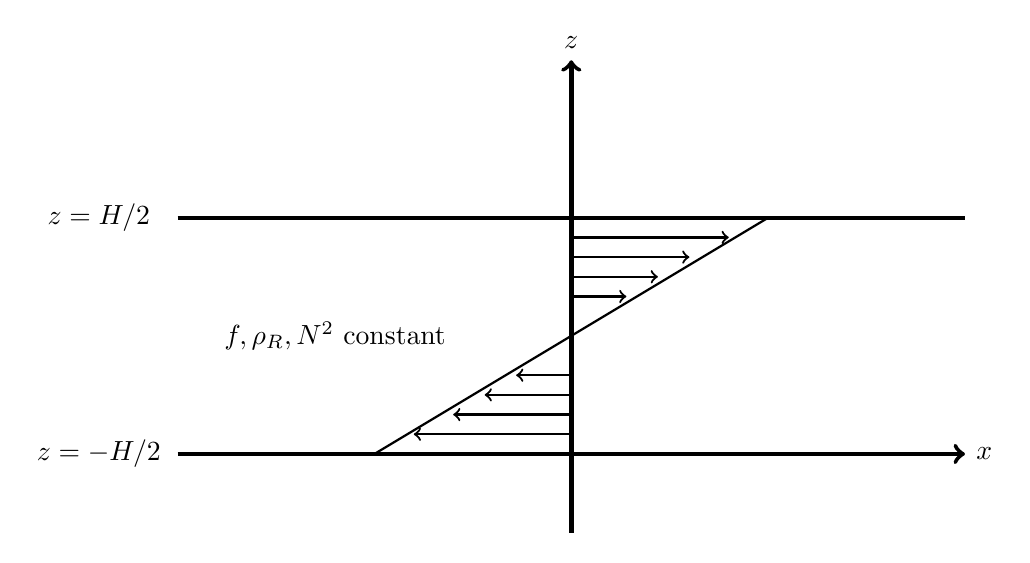
\begin{tikzpicture}
\draw[->,ultra thick] (-5,0)--(5,0) node[right]{$x$};
\draw[->,ultra thick] (0,-1)--(0,5) node[above]{$z$};
\draw[ultra thick] (-5,3)--(5,3); 
\draw[thick] (-2.5,0) -- (2.5,3);
\draw[thick,->] (0,2) -- (0.7,2);
\draw[thick,->] (0,2.25) -- (1.1,2.25);
\draw[thick,->] (0,2.5) -- (1.5,2.5);
\draw[thick,->] (0,2.75) -- (2,2.75);
\draw[thick,->] (0,1) -- (-0.7,1);
\draw[thick,->] (0,0.75) -- (-1.1,0.75);
\draw[thick,->] (0,0.5) -- (-1.5,0.5);
\draw[thick,->] (0,0.25) -- (-2,0.25);
\node at (-6,3) {$z = H/2$};
\node at (-6,0) {$z = -H/2$};
\node at (-3,1.5) {$f,\rho_R,N^2$ constant};
\end{tikzpicture}
  \caption{Sketch of the model described by Eady.}
  \label{eadyexample}
\end{figure}

\section{Cyclogenesis} 

\section{Summary}
\bibliography{references.bib}
\bibliographystyle{apa}

\end{document}
